%http://cms-results.web.cern.ch/cms-results/public-results/preliminary-results/SUS-16-024/index.html

%% CVSId: $Id: Example.tex,v 1.1.1.1 2000/11/28 11:15:12 exupery Exp $
\documentclass[%
xcolor=dvipsnames,table%,pdftex%,
%pdf,
%nocolorBG,
%colorBG,
%slideColor,
%slideBW,
%draft,
%frames
%azure
%contemporain
%nuancegris
%troispoints
%lignesbleues
%darkblue
%alienglow
%autumn
%12pt
]{beamer}
%%%%%%%%%%%%%%%%%%%%%%%%%%%%%
%\mode<presentation>
%{
  %\usetheme{Madrid}
 \usetheme[progressbar=frametitle]{m}% \usetheme{Boadilla}
  % or ...
%%%%%%%%%%%%%%%%%%%%%%%%%%%%%%%%%%%%%
%para revelar texto a aparecer en overlays
  %\setbeamercovered{transparent} 
  %\setbeamercovered{invisible}
%%%%%%%%%%%%%%%%%%%%%%%%%%%%%%%%%%%%%
  % \setbeamertemplate{blocks}[rounded][shadow=true]
  % \setbeamertemplate{navigation symbols}{}

  % \setbeamertemplate{footline}{%\hspace*{.5cm}
  %   \scriptsize{\phantom{Gg}%\insertauthor 
  %     \hspace*{50pt} 
  %     \hfill \insertframenumber
  %     \hspace*{.5cm}}}

  % % or whatever (possibly just delete it)
  % %\useoutertheme{shadow} 
  % \setbeamercolor{postit}{fg=black,bg=yellow}
  % \setbeamercolor{white}{fg=black,bg=white}
  % \setbeamercolor{cite}{fg=black,bg=yellow}
%}


\usepackage[absolute,overlay]{textpos}
\usepackage{booktabs}
\usepackage[scale=2]{ccicons}

%\usepackage{pgfplots}
%\usepgfplotslibrary{dateplot}

%%%%%%%%%%%%%%%%%%%%%%%%%%%%%%
%Force pdflatex processing even with "$ latex" (required by arXiv)
%\pdfoutput=1
\graphicspath{{figures/}}
%\usepackage[T1]{fontenc}
%\usepackage[utf8]{inputenc}
%\usepackage[spanish]{babel}
%\spanishdecimal{.}
%\usepackage{marvosym}
%\usepackage{beamerprosper}
\usepackage{amsmath,amssymb}
\usepackage{overpic}
\usepackage{graphicx}
\usepackage{mycolors}
%\usepackage{xmpmulti}
\usepackage{multimedia}
\usepackage{pgf}
\usepackage{cancel}
\usepackage{wasysym}
%\usepackage{helvet}
\usepackage{comment}
\usepackage{array}   % for \newcolumntype macro
\newcolumntype{L}{>{$}l<{$}} % math-mode version of "l" column type
\includecomment{comentar}
\specialcomment{comentar}
{\begingroup}{\medskip\endgroup}
\excludecomment{comentar}

\includecomment{comentario}
\specialcomment{comentario}
{\begingroup}{\endgroup}
\excludecomment{comentario}

\includecomment{details}
\specialcomment{details}
{\begingroup}{\endgroup}
\excludecomment{details}

%\usepackage[texcoord,grid,gridunit=mm,gridcolor=red!10,subgridcolor=green!10]{eso-pic}


\newcommand{\widescreen}{
\setlength{\paperwidth}{171 mm}
\setlength{\paperheight}{96 mm}
\setlength{\textwidth}{161 mm}
\setlength{\textheight}{86 mm}
}

%\widescreen


\title{Title}
\subtitle{Sibtitle  }


%\subtitle
%{Reconstruction of the neutrino mass matrix} % (optional)

\author{Diego Restrepo}
% - Use the \inst{?} command only if the authors have different
%   affiliation.
\institute{
  \begin{columns}
    \begin{column}{0.5\textwidth}
Instituto de F\'\i sica\\
Universidad de Antioquia\\
Phenomenology Group\\
\url{http://gfif.udea.edu.co}      
    \end{column}
    \begin{column}{0.5\textwidth}
      \hfill Image title\\
      \hfill 
\includegraphics[scale=0.15]{imageicon}\\
      \hfill \tiny{Image credits}
    \end{column}
  \end{columns}
\quad\\
\quad\\
{\tiny
\alert{\textbf{Focus on}} \\
arXiv:NNNN.NNNNN (Jrnl)\\
\alert{In collaboration with}\\
  N.~Name}
%\centering
}
% - Use the \inst command only if there are several affiliations.
% - Keep it simple, no one is interested in your street address.

\date{\tiny November 15, 2016 } % (optional) \today
%{
\includegraphics[scale=0.3]{udea}}
\titlegraphic{\hfill
\includegraphics[height=1.5cm]{udea}}

%\subject{Talks}
% This is only inserted into the PDF information catalog. Can be left
% out. 



% If you have a file called "university-logo-filename.xxx", where xxx
% is a graphic format that can be processed by latex or pdflatex,
% resp., then you can add a logo as follows:

% \pgfdeclareimage[height=0.5cm]{university-logo}{university-logo-filename}
% \logo{\pgfuseimage{university-logo}}



% Delete this, if you do not want the table of contents to pop up at
% the beginning of each subsection:
%\AtBeginSubsection[]
%{
%  \begin{frame}<beamer>
%    \frametitle{Outline}
%    \tableofcontents[currentsection,currentsubsection]
%  \end{frame}
%}

\newcommand{\chml}[2]{$\underline{\text{#1\hspace{#2}}}$}
\begin{document}


%===============
\begin{comentar}
%===============  
%=============
\end{comentar}
%=============

\maketitle
 % \begin{frame}%[plain]
 %   \titlepage
 % \end{frame}
% }

\end{document}

% {
% \usebackgroundtemplate{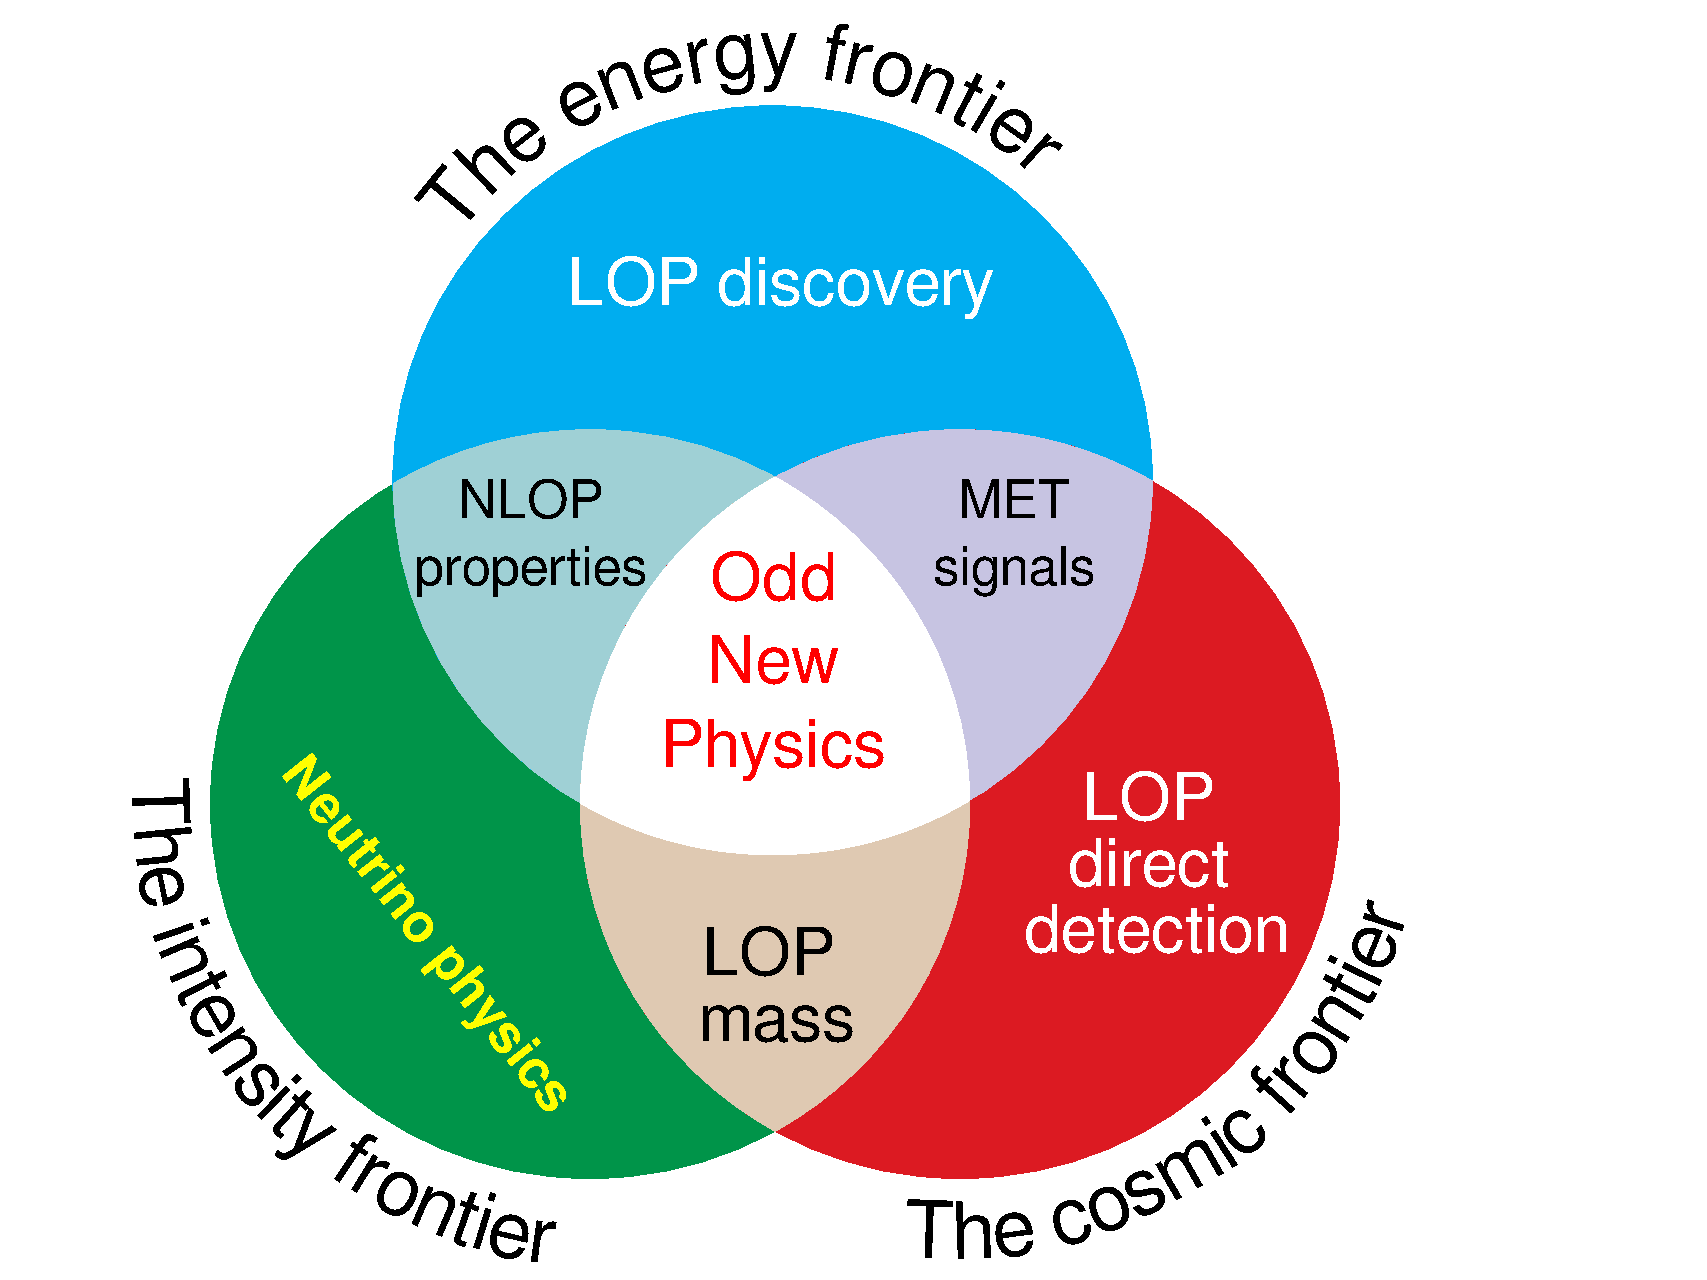
\includegraphics[width=\paperwidth]{tocrs}}
\begin{frame}
  \frametitle{Table of Contents}
\small
%\vspace{-0.5cm}
  \setbeamertemplate{section in toc}[sections numbered]
  \tableofcontents[hideallsubsections]
\end{frame}


\section{First section}

% * <restrepo@udea.edu.co> 2015-11-15T12:41:09.269Z:
%
% Rememeber the basic idea: combine nu and dark matter
%
% ^.

\begin{frame}
  \frametitle{First slide}

\end{frame}
%%%%%


\section{Second section}
%%%%
\begin{frame}

\end{frame}
\end{document}





TEMPLATES

1. Background image slide
%%%%%%%%%%%%%%%%%%%%%%%%%%%%%%
{
\usebackgroundtemplate{\includegraphics[width=\paperwidth]{file}}
\setbeamertemplate{blocks}[rounded][shadow=false]
\setbeamercovered{invisible}
\begin{frame}[plain]
\end{frame}
}
%%%%%%%%%%%%%%%%%%%%%%%%%%%%%%

2. Two columns
\begin{columns}
  \begin{column}{0.48\textwidth}
    
  \end{column}
  \begin{column}{0.48\textwidth}
    
  \end{column}
\end{columns}




\begin{columns}
  \column{.48\textwidth}
  \begin{block}<2->{}
  \end{block}
  \column{.48\textwidth}
  \begin{block}<2->{}
  \end{block}
\end{columns}

%%%%%%%%%%%%%%%%%%%%%
{
\usebackgroundtemplate{\includegraphics[width=\paperwidth]{file}}
\setbeamertemplate{blocks}[rounded][shadow=false]
\setbeamercovered{invisible}
\begin{frame}[plain]
  \begin{block}{}
    Name
  \end{block}
\end{frame}
}
%%%%
{
\usebackgroundtemplate{\includegraphics[width=\paperwidth]{file}}
\setbeamertemplate{blocks}[rounded][shadow=false]
\setbeamercovered{invisible}
\begin{frame}[plain]
\end{frame}
%%%%%%%%%%%%%%%%%%
}


%Trick to put stuff in specfic places of an slide:
\begin{frame}
\begin{picture}(320,250)
\put(-25,190){D.R. \emph{et al}: arXiv:1006.5075 [PRD]\qquad\qquad arXiv:1206.3605 [PRD]}
\put(-37,20){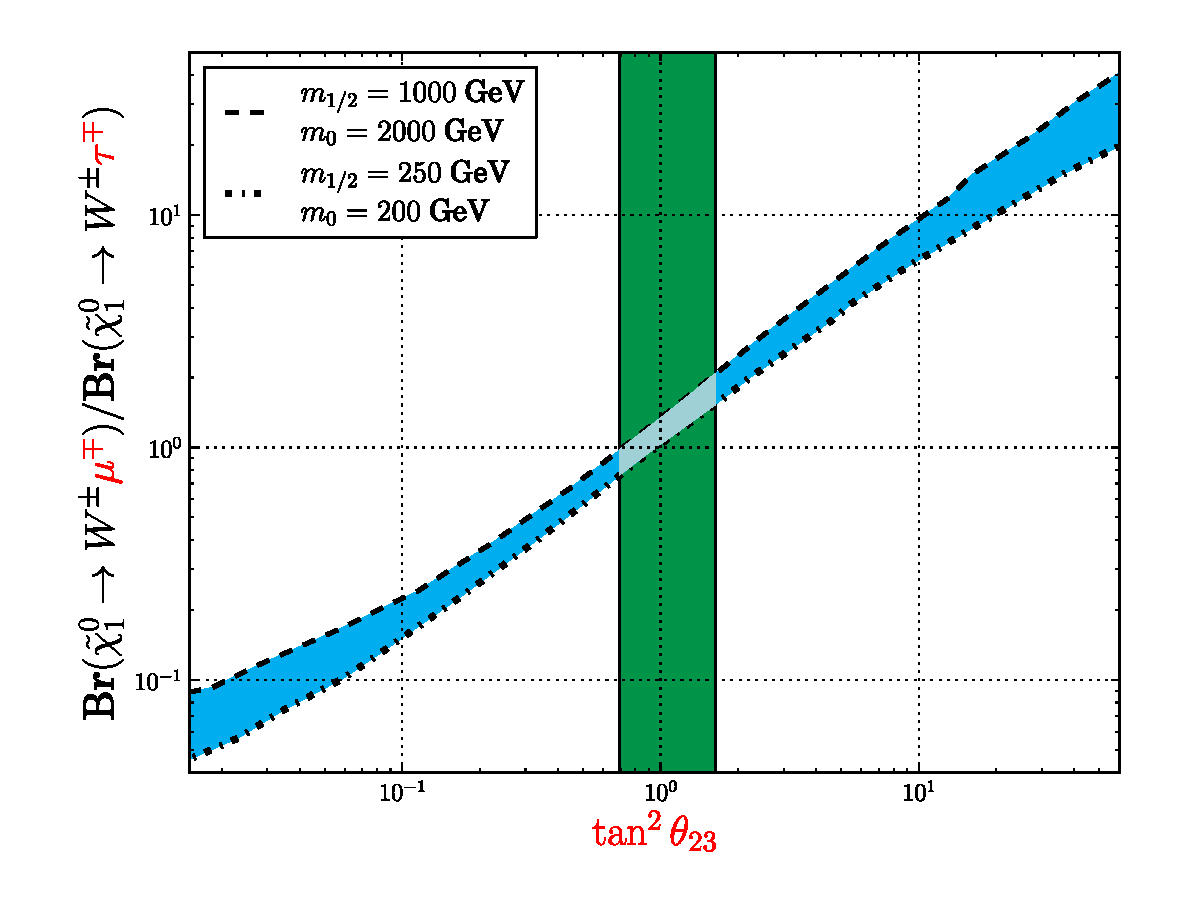
\includegraphics[scale=0.35]{atmcorrelationm}}
\put(143,20){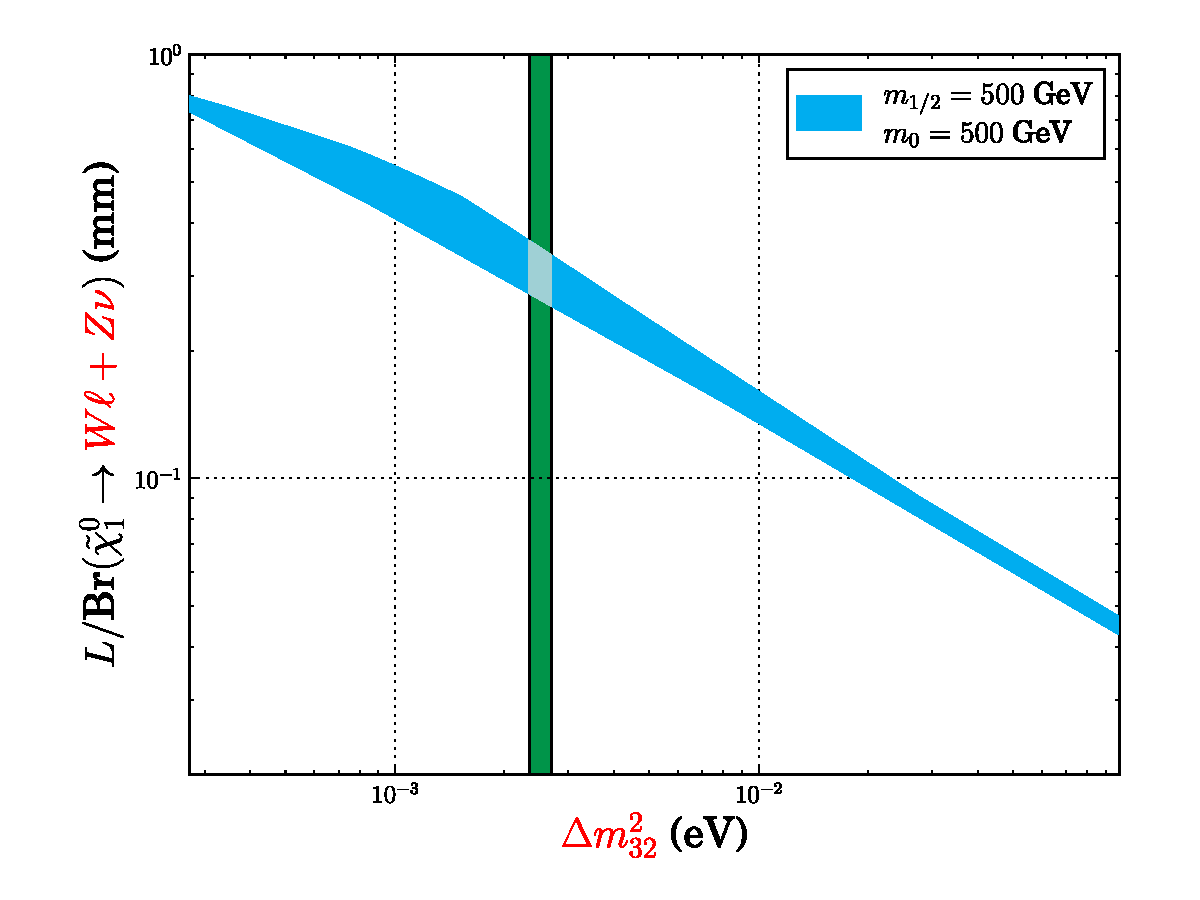
\includegraphics[scale=0.35]{LoverWlZnu_Dm23_500_500_randomm}}
\put(0,160){Only depend in \alert{$\Lambda_i$}}
\end{picture}
\end{frame}
%%%%%
Background like
%%%%%%%%%%%%%%%%%%%%%%%%
\begin{frame}[plain]
\begin{picture}(320,250)
\only<1>{\put(-30,-15){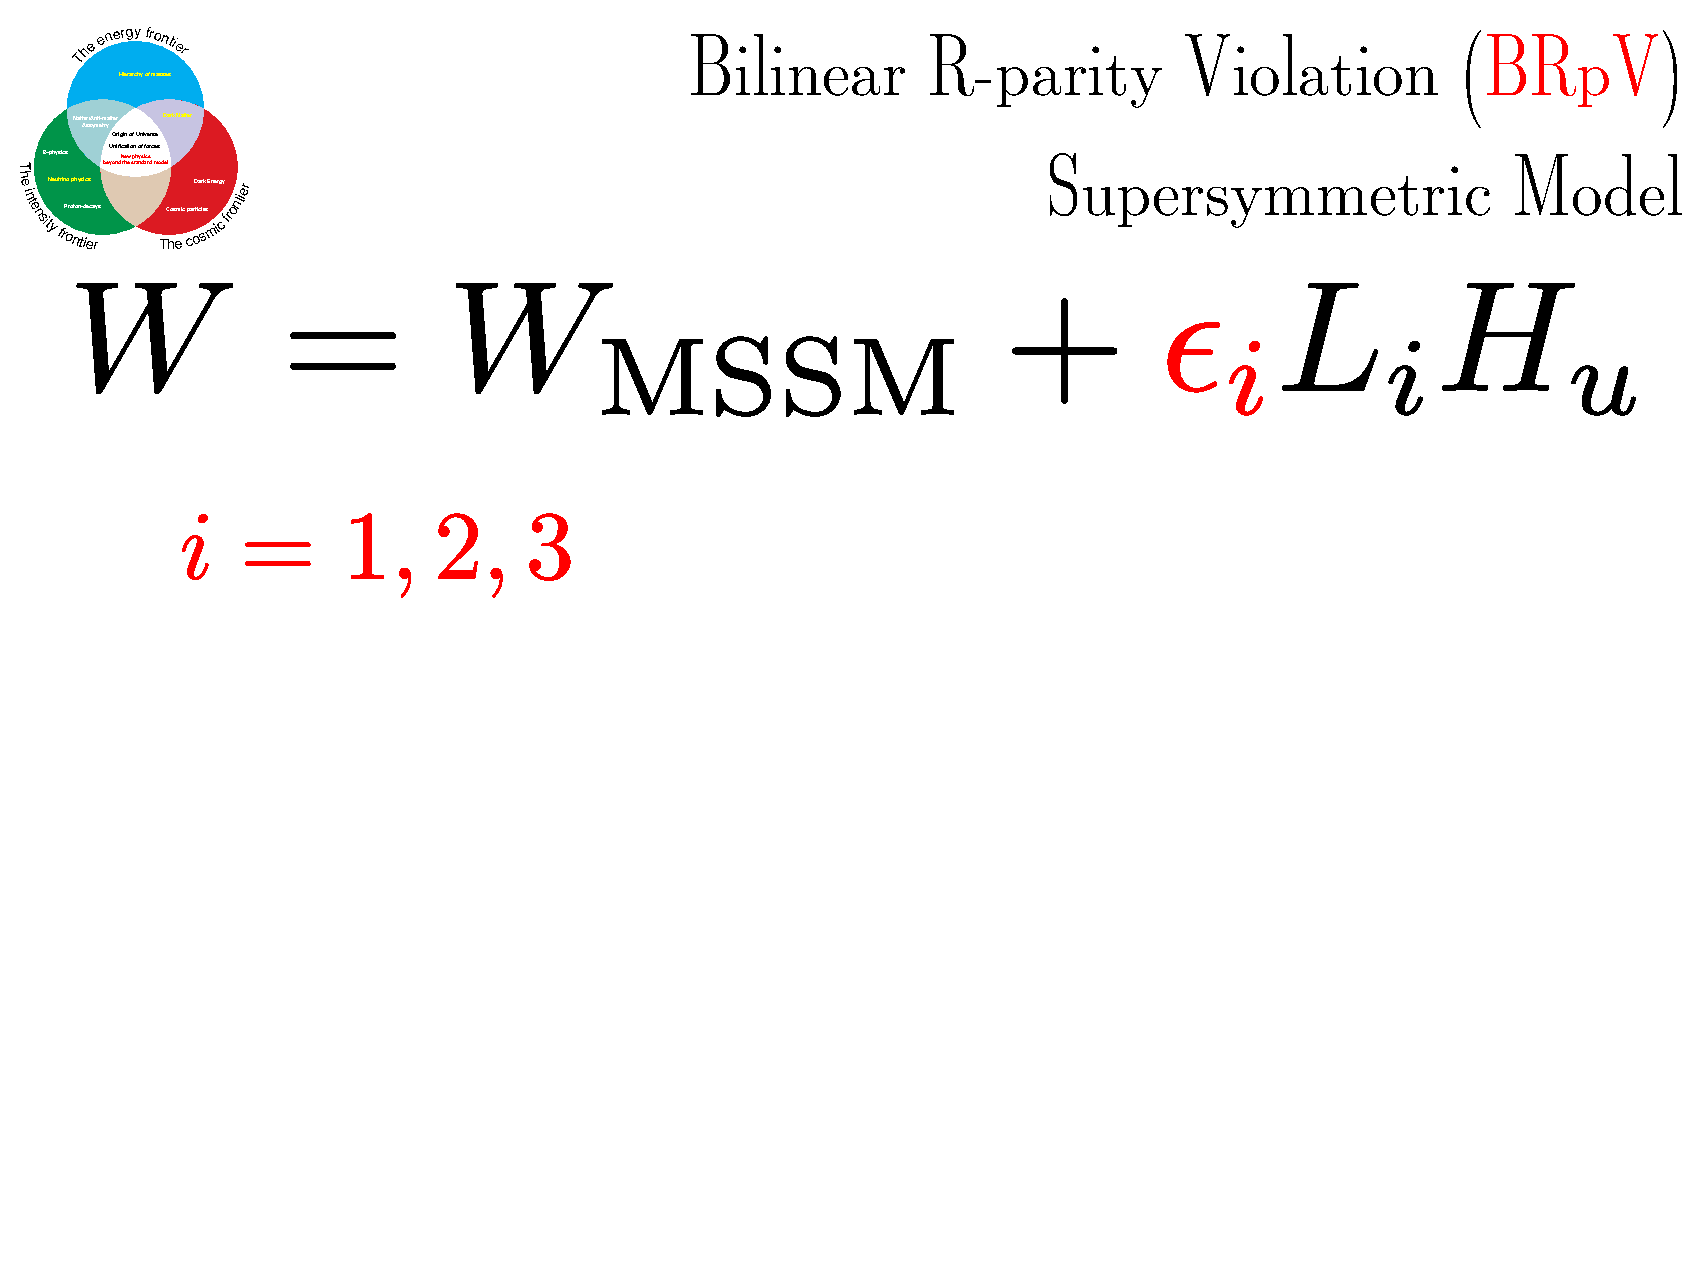
\includegraphics[width=\paperwidth]{brpv1}}}%
\only<2>{\put(-30,-15){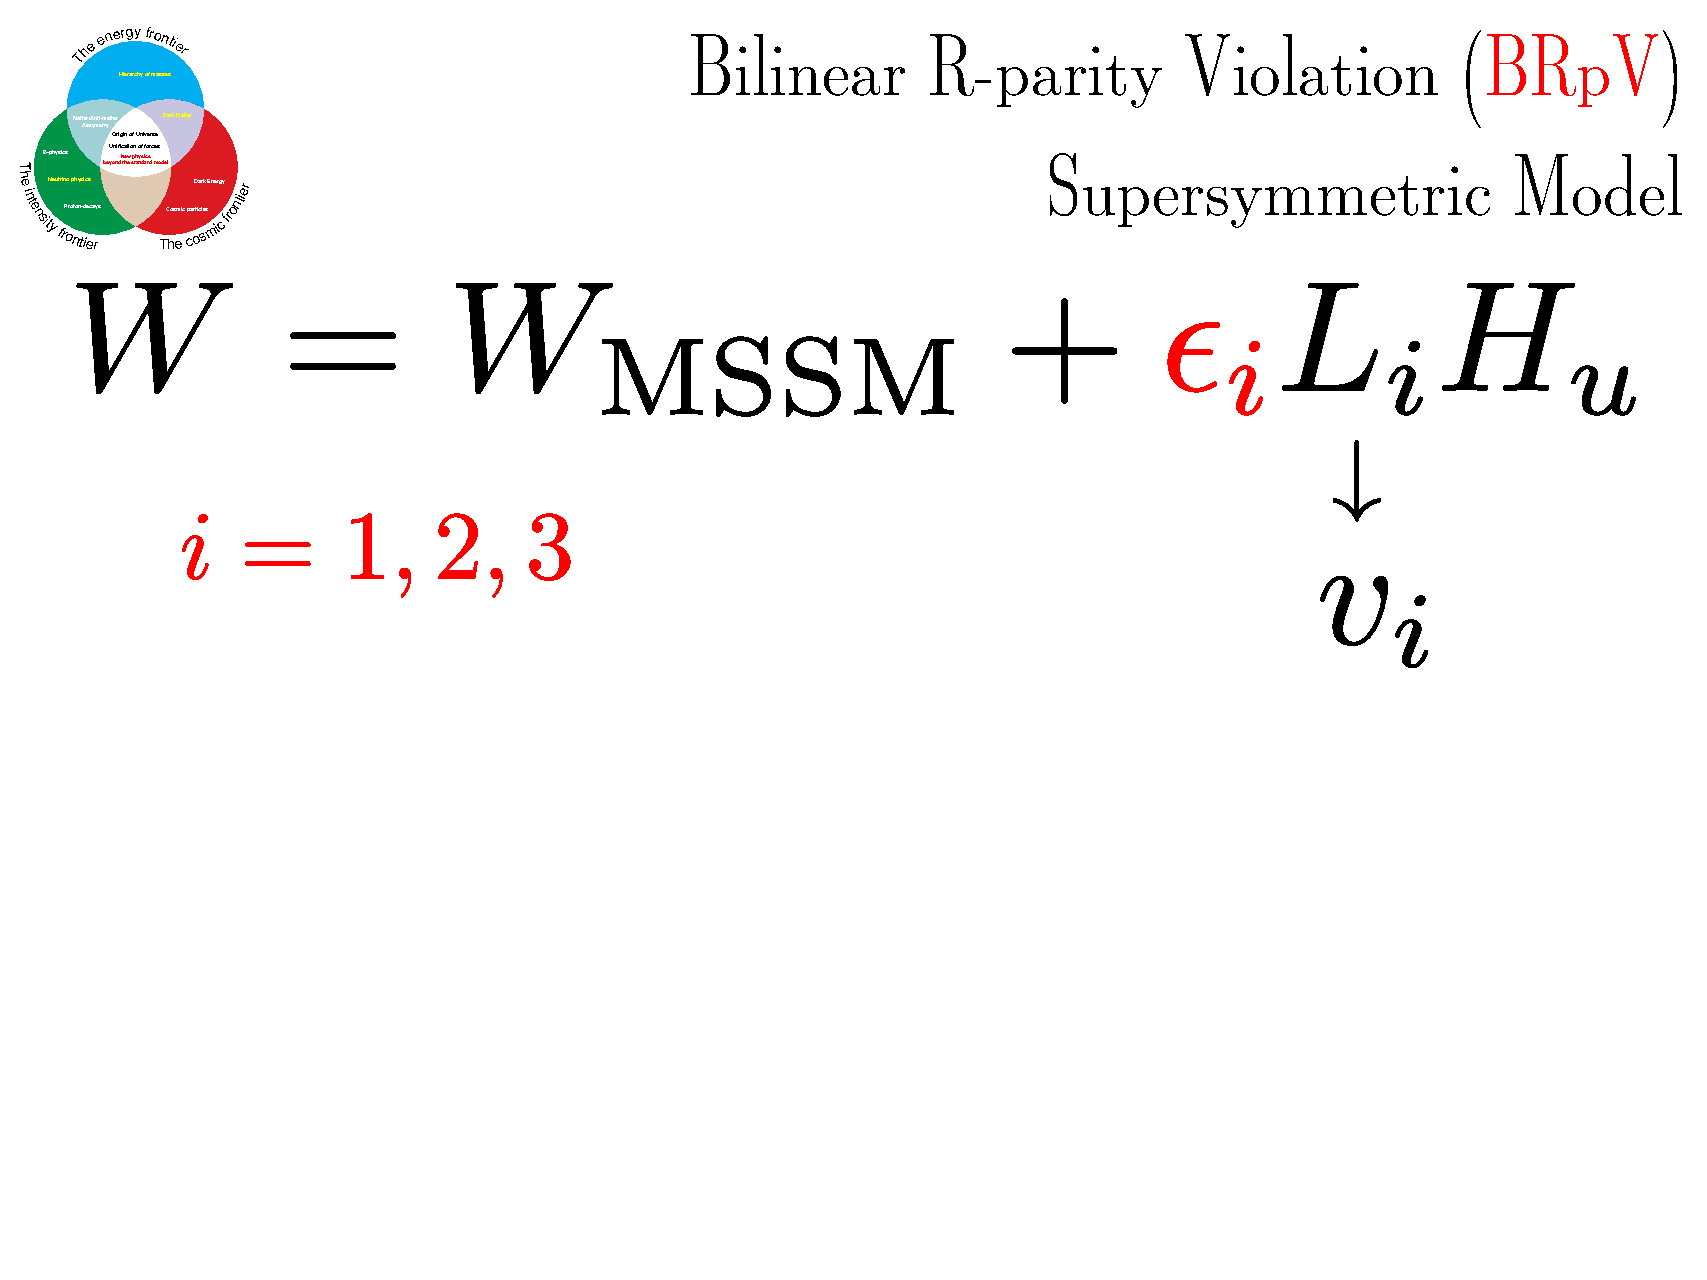
\includegraphics[width=\paperwidth]{brpv2}}}%    
\only<2>{\put(-30,-15){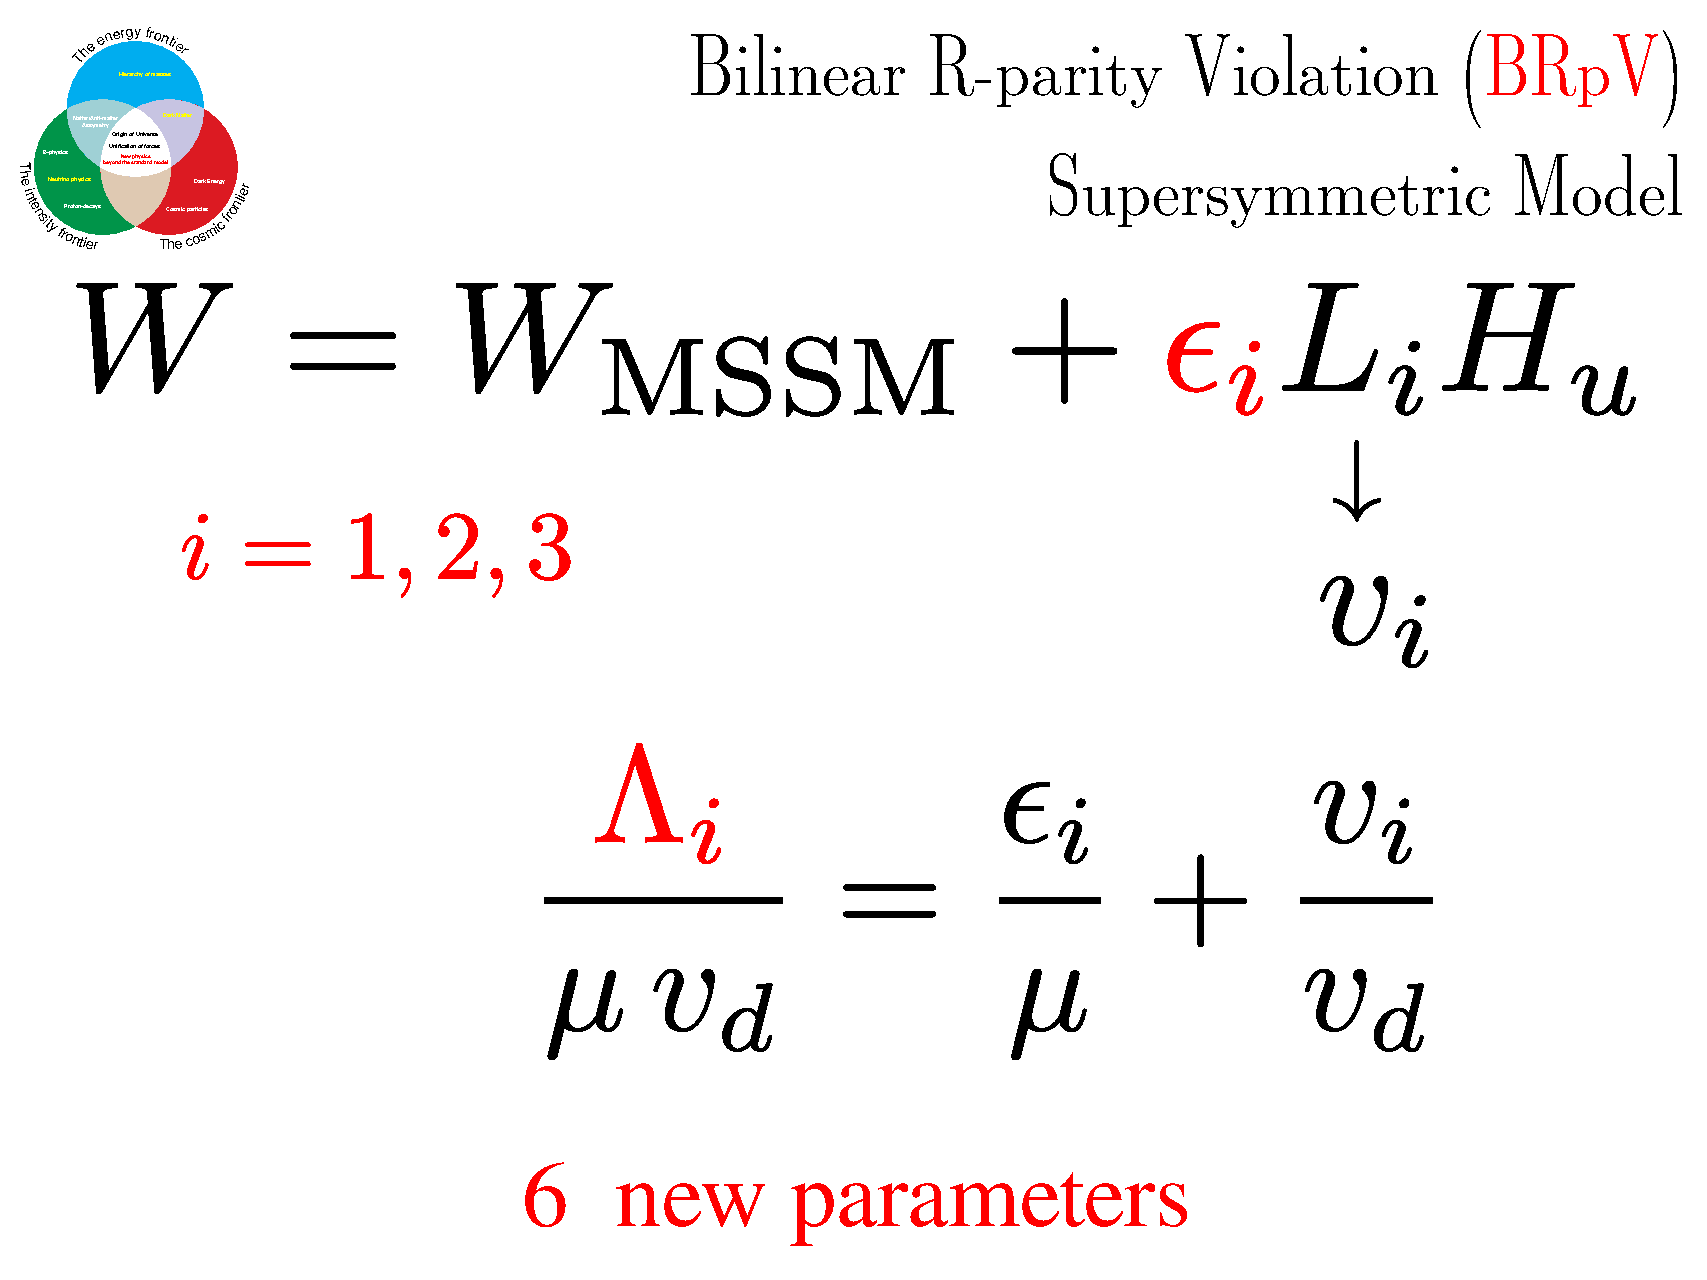
\includegraphics[width=\paperwidth]{brpv3}}}%    
\end{picture}
\end{frame}


%%%
Post it

\setbeamercolor{postit}{fg=black,bg=yellow}
\begin{beamercolorbox}[sep=1em,wd=5cm]{postit}
Place me somewhere!
\end{beamercolorbox}

%%%combine with textblock
\begin{textblock*}{297mm}(0mm,0mm)%
\begin{beamercolorbox}[sep=0.1em,wd=4cm,center,rounded=true,shadow=true]{cite}
\scriptsize Akhmedov, hep-ph/0001264
\end{beamercolorbox}
\end{textblock*}

%%More colorboxes
\setlength{\fboxrule}{3 pt}
\fcolorbox{red}{yellow}{caja de fondo
amarillo y contorno rojo}\\
\setlength{\fboxsep}{5pt}
\fcolorbox{red}{yellow}{caja de fondo
amarillo y contorno rojo}

\only<11>{\put(-20,80){
\begin{minipage}[t]{1.0\linewidth}
%\metroset{block=fill}
\begin{block}{SM particles}
     Gauge invariance+Lorentz Invariance$\to$Lagrangian (interactions)   
\end{block}
    \end{minipage}
}}


\begin{frame}
\begin{picture}(320,250)
\only<1->{\put(0,100){
  \begin{overpic}[scale=0.4,grid
            ]{table1}
\put(40,38){\tikz \draw[red,thick,rounded corners] (0,0) rectangle (2,0.5);}
  \end{overpic}
}
}
%%%circle
\end{picture}
\end{frame}
